\documentclass{standalone}
\usepackage{tikz}
\usetikzlibrary{matrix, shapes.multipart, positioning}

\begin{document}
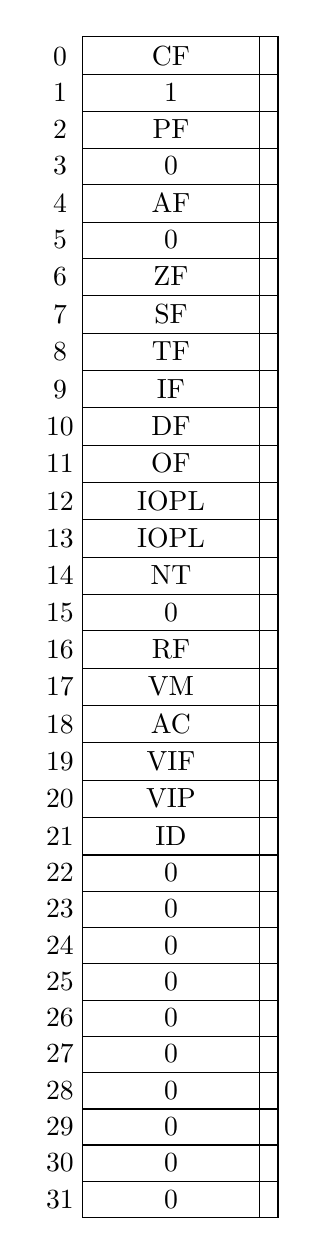
\begin{tikzpicture}

\matrix (m1) [ matrix of nodes, nodes in empty cells, column sep=0, row sep=0,
column 1/.style={},
column 2/.style={nodes={text width=2cm, align=center}}] {
0	&CF& \\
1	&1 &\\
2	&PF& \\
3	&0 &\\
4	&AF&\\
5	&0 &\\
6	&ZF &\\
7	&SF &\\
8	&TF	&\\
9	&IF	&\\
10	&DF	&\\
11	&OF	&\\
12	&IOPL &\\
13	&IOPL &\\
14	&NT	&\\
15	&0	&\\
16	&RF	&\\
17	&VM	&\\
18	&AC &\\
19	&VIF	&\\
20	&VIP &\\
21	&ID	&\\
22	&0	&\\
23	&0	&\\
24	&0	&\\
25	&0	&\\
26	&0	&\\
27	&0	&\\
28	&0	&\\
29	&0	&\\
30	&0	&\\
31	&0	&\\
};

\draw (m1-1-2.north west) rectangle (m1-32-2.south east);
\draw (m1-1-2.north east) rectangle (m1-32-3.south east);
\draw (m1-31-2.north west) rectangle (m1-32-2.south east);
\draw (m1-31-2.north east) rectangle (m1-32-3.south east);

\foreach \x in {1,2,...,31}{ \draw (m1-\x-2.south west) -- (m1-\x-3.south east); }

\end{tikzpicture}
\end{document}